%!TEX TX-program = xelatex
%
%%%%%%%%%%%%%%%%%%%%
%
% Title: GCSE Mathematics & Additional Mathematics for 08.09.22 (2)
% Author: Eason Shao, Mr Finch-Noyes
% Date: 08.09.22 (2)
% Institude: Oxford International College
% Email: eason.syc@icloud.com; yicheng_shao@oxcoll.com
% GitHub: https://github.com/EasonSYC
% GitHub Repository: https://github.com/EasonSYC/GCSE-Maths-Notes
%
%%%%%%%%%%%%%%%%%%%%

\documentclass[8pt]{article}
\usepackage{../allan-eason}

\usetikzlibrary{positioning}
\usetikzlibrary{svg.path}

\graphicspath{ {./images/} }

\newcommand{\Date}{08.09.22 (2)}
\newcommand{\Name}{Mathematics}
\newcommand{\Title}{\textcolor{allandarkblue}{\Name}\ \textcolor{allancyan}{\Date}\ Notes}

\newcommand{\Author}{Eason Shao, Mr Finch-Noyes}

\author{\Author}
\title{\Title}
\date{\Date}

\geometry{a4paper, scale=0.8}

\lhead{\Title}

\begin{document}

	\maketitle

	\tableofcontents

	\section{Linear Graph}
		\subsection{Sketching a Graph}
			\defi \defiword{(Plot and Sketch)} \defiword{Plot} needs to be accurate (e.g. scale), \defiword{Sketch} can be not so accurate (Focus on Shape).

			\exmp \exmpword{(Plot)} Plot \(y = 3x + 1\).

			\begin{center}
				\begin{tabular}{c|cccc}
					\(x\) & \(5\) & \(0\) & \(1\) & \(-2\)\\
					\hline
					\(y\) & \(16\) & \(1\) & \(4\) & \(-5\)\\
				\end{tabular}
			\end{center}

			\begin{center}
				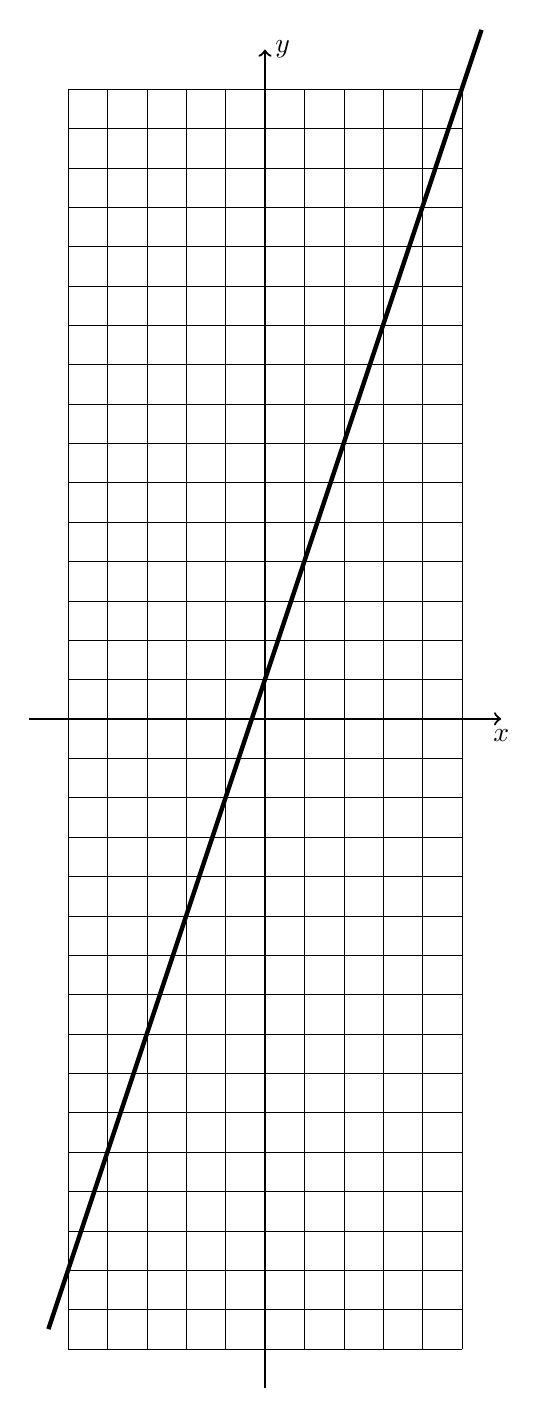
\begin{tikzpicture}[scale = 0.5]
					\draw [black, thick, ->] (-6, 0) -- (6, 0) node[below] {\(x\)};
					\draw [black, thick, ->] (0, -17) -- (0, 17) node[right] {\(y\)};
					\draw [step = 1.0, black, ultra thin] (-5, -16) grid (5, 16);
					\draw [black, domain = -5.5 : 5.5, ultra thick] plot (\x, {3 * \x + 1});
				\end{tikzpicture}
			\end{center}

			\exmp \exmpword{(Sketch)} Sketch \(y = 2x - 1\). Meet \(x\) axis at \((1/2, 0)\); Meets \(y\) axis at \((0, -1)\).

			\begin{center}
				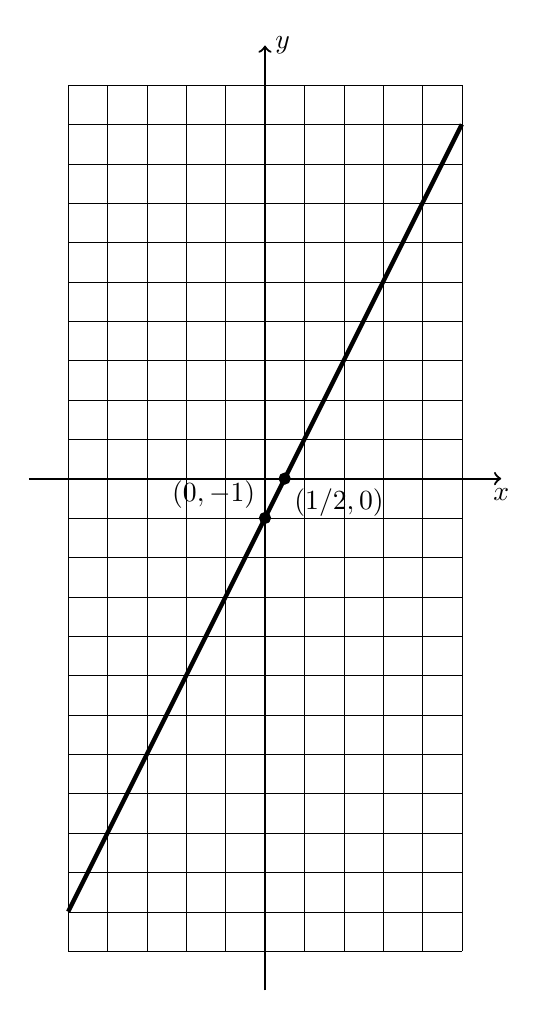
\begin{tikzpicture}[scale = 0.5]
					\draw [black, thick, ->] (-6, 0) -- (6, 0) node [below] {\(x\)};
					\draw [black, thick, ->] (0, -13) -- (0, 11) node [right] {\(y\)};
					\draw [step = 1.0, black, ultra thin] (-5, -12) grid (5, 10);
					\draw [black, domain = -5 : 5, ultra thick] plot (\x, {2 * \x - 1});
					\node at (0.5, 0) [anchor = north west] {\((1/2, 0)\)};
					\draw [black, fill = black] (0.5, 0) circle (4pt);
					\draw [black, fill = black] (0, -1) circle (4pt);
					\node at (0, -1) [anchor = south east] {\((0, -1)\)};
				\end{tikzpicture}
			\end{center}

			\prob Sketch \(y = x + 3\).
			
			\solution Meet \(x\) axis at \((-3, 0)\); Meets \(y\) axis at \((0, 3)\).

			\begin{center}
				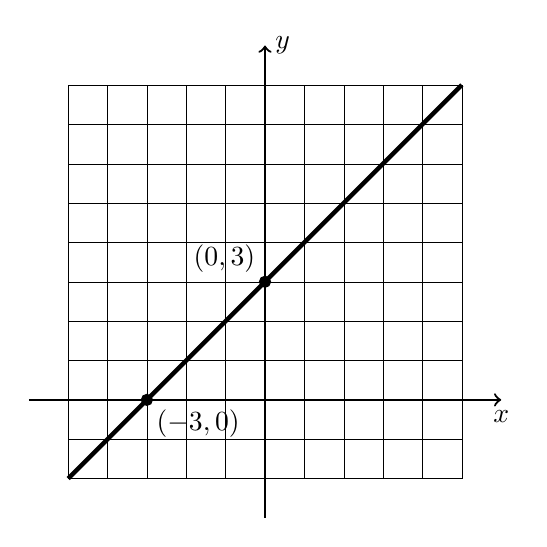
\begin{tikzpicture}[scale = 0.5]
					\draw [black, thick, ->] (-6, 0) -- (6, 0) node [below] {\(x\)};
					\draw [black, thick, ->] (0, -3) -- (0, 9) node [right] {\(y\)};
					\draw [step = 1.0, black, ultra thin] (-5, -2) grid (5, 8);
					\draw [black, domain = -5 : 5, ultra thick] plot (\x, {\x + 3});
					\node at (-3, 0) [anchor = north west] {\((-3, 0)\)};
					\draw [black, fill = black] (-3, 0) circle (4pt);
					\node at (0, 3) [anchor = south east] {\((0, 3)\)};
					\draw [black, fill = black] (0, 3) circle (4pt);
				\end{tikzpicture}
			\end{center}

			\prob Sketch \(y = -2x + 1\).
			
			\solution Meet \(x\) axis at \((1/2, 0)\); Meets \(y\) axis at \((0, 1)\).

			\begin{center}
				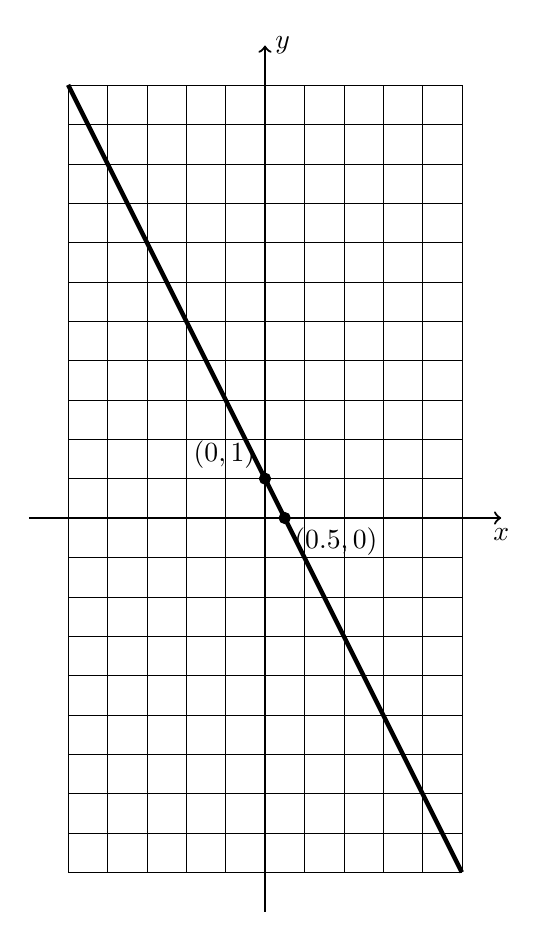
\begin{tikzpicture}[scale = 0.5]
					\draw [black, thick, ->] (-6, 0) -- (6, 0) node [below] {\(x\)};
					\draw [black, thick, ->] (0, -10) -- (0, 12) node [right] {\(y\)};
					\draw [step = 1.0, black, ultra thin] (-5, -9) grid (5, 11);
					\draw [black, domain = -5 : 5, ultra thick] plot (\x, {-2 * \x + 1});
					\node at (0.5, 0) [anchor = north west] {\((0.5, 0)\)};
					\draw [black, fill = black] (0.5, 0) circle (4pt);
					\node at (0, 1) [anchor = south east] {\((0, 1)\)};
					\draw [black, fill = black] (0, 1) circle (4pt);
				\end{tikzpicture}
			\end{center}

			\prob Sktech \(y = 1/2 x\).

			\solution Meet \(x\) and \(y\) axis at Origin \((0, 0)\).
			
			\begin{center}
				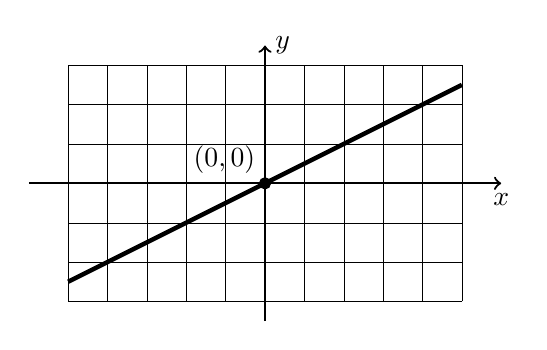
\begin{tikzpicture}[scale = 0.5]
					\draw [black, thick, ->] (-6, 0) -- (6, 0) node [below] {\(x\)};
					\draw [black, thick, ->] (0, -3.5) -- (0, 3.5) node [right] {\(y\)};
					\draw [step = 1.0, black, ultra thin] (-5, -3) grid (5, 3);
					\draw [black, domain = -5 : 5, ultra thick] plot (\x, {0.5 * \x});
					\node at (0, 0) [anchor = south east] {\((0, 0)\)};
					\draw [black, fill = black] (0, 0) circle (4pt);
				\end{tikzpicture}
			\end{center}

			\prob Sketch \(y = 7\).
			
			\solution 

			\begin{center}
				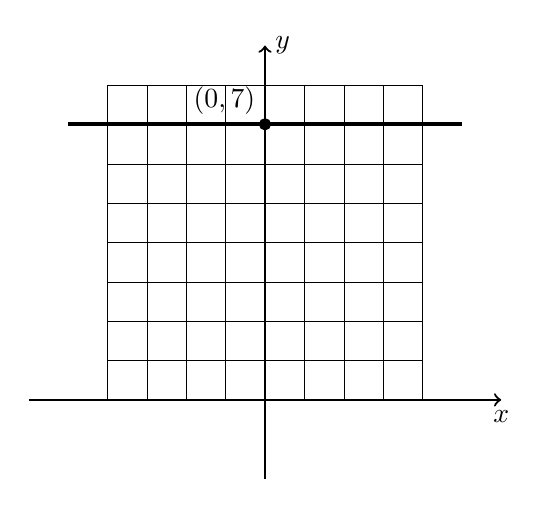
\begin{tikzpicture}[scale = 0.5]
					\draw [black, thick, ->] (-6, 0) -- (6, 0) node [below] {\(x\)};
					\draw [black, thick, ->] (0, -2) -- (0, 9) node [right] {\(y\)};
					\draw [step = 1.0, black, ultra thin] (-4, 0) grid (4, 8);
					\draw [black, domain = -5 : 5, ultra thick] plot (\x, 7);
					\node at (0, 7) [anchor = south east] {\((0, 7)\)};
					\draw [black, fill = black] (0, 7) circle (4pt);
				\end{tikzpicture}
			\end{center}

			\prob Sketch \(x = 2\).
			
			\solution 

			\begin{center}
				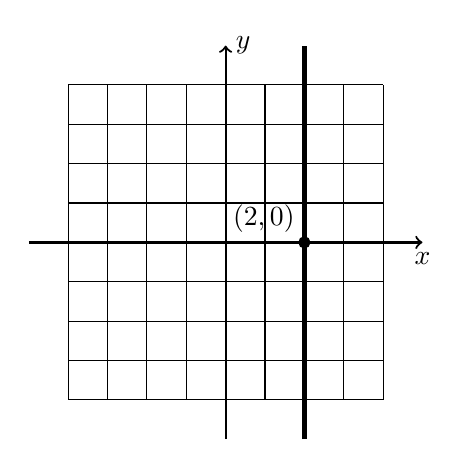
\begin{tikzpicture}[scale = 0.5]
					\draw [black, thick, ->] (-5, 0) -- (5, 0) node [below] {\(x\)};
					\draw [black, thick, ->] (0, -5) -- (0, 5) node [right] {\(y\)};
					\draw [step = 1.0, black, thin] (-4, -4) grid (4, 4);
					\draw [black, ultra thick] (2, -5) -- (2, 5);
					\node at (2, 0) [anchor = south east] {\((2, 0)\)};
					\draw [black, fill = black] (2, 0) circle (4pt);
				\end{tikzpicture}
			\end{center}

			\prob Sketch \(2x + y = 10\).
			
			\solution Meet \(x\) axis at \((5, 0)\); Meet \(y\) axis at \((0, 10)\).

			\begin{center}
				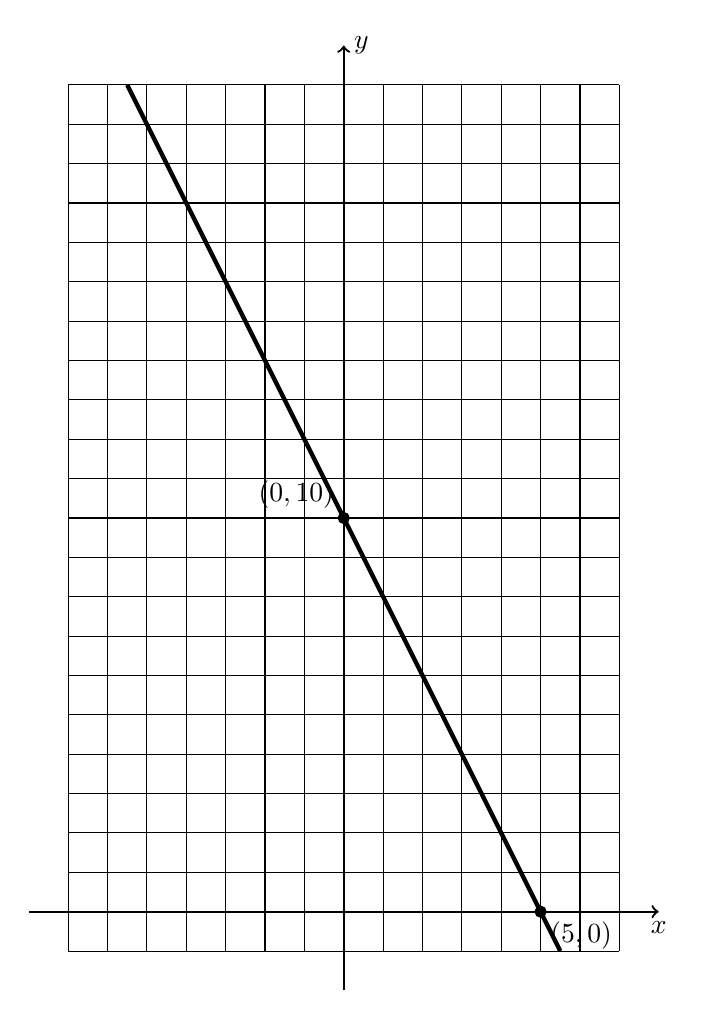
\begin{tikzpicture}[scale = 0.5]
					\draw [black, thick, ->] (-8, 0) -- (8, 0) node [below] {\(x\)};
					\draw [black, thick, ->] (0, -2) -- (0, 22) node [right] {\(y\)};
					\draw [step = 1.0, black, thin] (-7, -1) grid (7, 21);
					\draw [black, domain = -5.5 : 5.5, ultra thick] plot (\x, {10 - 2 * \x});
					\draw [black, fill = black] (5, 0) circle (4pt);
					\node at (5, 0) [anchor = north west] {\((5, 0)\)};
					\draw [black, fill = black] (0, 10) circle (4pt);
					\node at (0, 10) [anchor = south east] {\((0, 10)\)};
				\end{tikzpicture}
			\end{center}

			\prob Sketch \(x + 3y + 6 = 0\).
			
			\solution Meet \(x\) axis at \((-6, 0)\); Meet \(y\) axis at \((0, -2)\).

			\begin{center}
				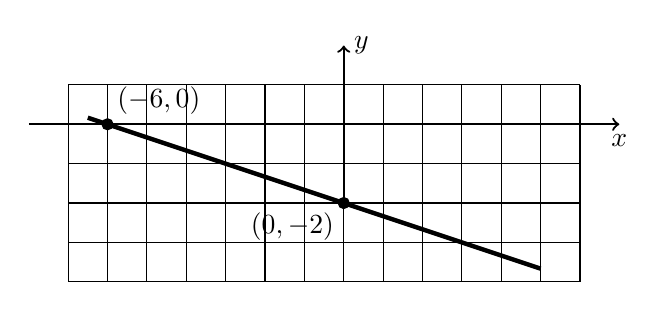
\begin{tikzpicture}[scale = 0.5]
					\draw [black, thick, ->] (-8, 0) -- (7, 0) node [below] {\(x\)};
					\draw [black, thick, ->] (0, -2) -- (0, 2) node [right] {\(y\)};
					\draw [step = 1.0, black, thin] (-7, 1) grid (6, -4);
					\draw [black, domain = -6.5 : 5, ultra thick] plot (\x, {-2 - \x / 3});
					\draw [black, fill = black] (-6, 0) circle (4pt);
					\node at (-6, 0) [anchor = south west] {\((-6, 0)\)};
					\draw [black, fill = black] (0, -2) circle (4pt);
					\node at (0, -2) [anchor = north east] {\((0, -2)\)};
				\end{tikzpicture}
			\end{center}

			\prob Sketch \(x = 0\).

			\solution \(y\) axis. \methword{Not \(x\) axis!}

			\prob Sketch \(y = 0\).

			\solution \(x\) axis. \methword{Not \(y\) axis!}

			\prob Sketch \(x + y = 0\).

			\solution \(y = -x\).

		\subsection{Use of Graphs}
			\meth \methword{(Using Graphs to Solve Equations)} A equation \(f(x) = g(x)\) can be solved using plotting graphs of \(f(x)\) and \(g(x)\) and checking the intersectinos.

			\prob Determine the number of solutions to the equation

			\[
				\frac{1}{(x-1)^5} = x,
			\]

			and determine the approximate values of each solution.

			\solution Sketch the graphs:

			\begin{center}
				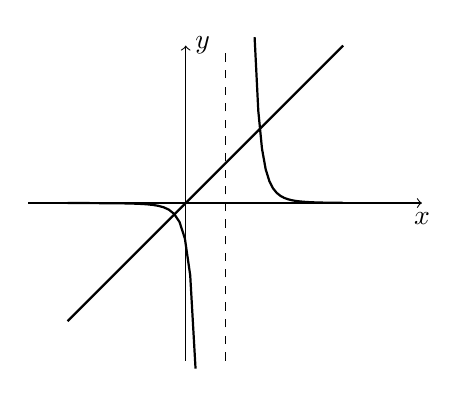
\begin{tikzpicture}[scale = 0.5]
					\draw [black, ->] (-4, 0) -- (6, 0) node [below] {\(x\)};
					\draw [black, ->] (0, -4) -- (0, 4) node [right] {\(y\)};
					\draw [black, dashed] (1, -4) -- (1, 4);
					\draw [black, domain = -3 : 0.25, thick] plot (\x, {1 / (\x - 1) ^ 5});
					\draw [black, domain = 1.75 : 4, thick] plot (\x, {1 / (\x - 1) ^ 5});
					\draw [black, domain = -3 : 4, thick] plot (\x, \x);
				\end{tikzpicture}
			\end{center}

			Two solutions (two intersections), one slightly smaller than \(0\), one bigger than \(1\) and close to \(2\).

		\subsection{Gradient}
			\defi \defiword{(Gradient in a Linear Graph)} Change in \(y\) when \(x\) increases by \(1\).

			\exmp \exmpword{(Gradient)} Work out the gradient of the line below.

			\exmp \exmpword{(Gradient)} Work out the gradient of the line below.

			\prob Calculate the following four gradients.
				\begin{enumerate}[label = \probword{(\arabic*)}]
					\item 
					\[
						\begin{tikzpicture}[scale = 0.5]
							\draw [black, ->] (-10, 0) -- (10, 0) node [below] {\(x\)};
							\draw [black, ->] (0, -10) -- (0, 10) node [right] {\(y\)};
							\draw [black, domain = -8 : 8] plot (\x, {0.5 * \x + 1.5});
							\draw [black, fill = black] (1, 2) circle (3pt) node [anchor = north east] {\((1, 2)\)};
							\draw [black, fill = black] (7, 5) circle (3pt) node [anchor = north west] {\((7, 5)\)};
						\end{tikzpicture}
					\]

					\solution \(m = (5-2)/(7-1) = 1/2\).

					\item 
					\[
						\begin{tikzpicture}[scale = 0.25]
							\draw [black, ->] (-10, 0) -- (10, 0) node [below] {\(x\)};
							\draw [black, ->] (0, -20) -- (0, 20) node [right] {\(y\)};
							\draw [black, domain = -4 : 4] plot (\x, {-6 * \x + -1});
							\draw [black, fill = black] (-1, 5) circle (3pt) node [anchor = north west] {\((-1, 5)\)};
							\draw [black, fill = black] (3, -19) circle (3pt) node [anchor = north west] {\((3, -19)\)};
						\end{tikzpicture}
					\]

					\solution \(m = (-19-5)/(3--1) = -6\).

					\item 
					\[
						\begin{tikzpicture}[scale = 0.2]
							\draw [black, ->] (-40, 0) -- (40, 0) node [below] {\(x\)};
							\draw [black, ->] (0, -15) -- (0, 15) node [right] {\(y\)};
							\draw [black, domain = -35 : 35] plot (\x, {- \x / 3});
							\draw [black, fill = black] (30, -10) circle (3pt) node [anchor = north east] {\((30, -10)\)};
						\end{tikzpicture}
					\]

					\solution \(m = (-10)/30 = -1/3\).

					\item 
					\[
						\begin{tikzpicture}[scale = 0.25]
							\draw [black, ->] (-10, 0) -- (10, 0) node [below] {\(x\)};
							\draw [black, ->] (0, -5) -- (0, 5) node [right] {\(y\)};
							\draw [black, domain = -8 : 8] plot (\x, 2);
							\draw [black, fill = black] (-4, 2) circle (3pt) node [anchor = north east] {\((-4, 2)\)};
							\draw [black, fill = black] (5, 2) circle (3pt) node [anchor = north east] {\((5, 2)\)};
						\end{tikzpicture}
					\]

					\solution \(m = 0\).

				\end{enumerate}

			\meth \methword{(Calculating Gradient)} Gradient \(m = (y_2 - y_1)/(x_2 - x_1)\)

		\subsection{Writing an Equation}
			\defi \defiword{(Linear Equation)} \(y = mx + C\). \(m\) is the \defiword{Gradient} and \(C\) is the \defiword{\(y\)-intercept}.

			\prob Write the equations of the previous four lines.

			\solution

			\begin{enumerate}[label = \methword{(\arabic*)}]
				\item \(y = 1/2 x + C\), let \((x, y) = (1, 2)\), \(c = 3/2\), \(y = 1/2 x + 3/2\).
				\item \(y = -6 x + C\), let \((x, y) = (-1, 5)\), \(c = -1\), \(y = -6x - 1\).
				\item \(y = -1/3 x + C\), let \((x, y) = (0, 0)\), \(c = 0\), \(y = -1/3 x\).
				\item \(y = C\), \(y = 2\).
			\end{enumerate}

		\subsection{Parallel and Perpendicular}
			\meth \methword{(Parallel)} Two \methword{parallel} lines have the same gradient or if they both have undefined gradient (i.e. verticle). That is, for \(l_1: y = m_1 x + c_1, l_2: y = m_2 x + c_2, m_1 = m_2 \Leftrightarrow l_1 \parallel l_2\).

			\meth \methword{(Perpendicular)} Two \methword{perpendicular} lines have gradient with the product of \(-1\) or one is \(0\) and one is undefined. That is, for \(l_1: y = m_1 x + c_1, l_2: y = m_2 x + c_2, m_1 \times m_2 = -1 \Leftrightarrow l_1 \perp l_2\).

			\prob Prove the relationship between the product of gradients and being perpendicular.

			\solution Let \(l_1: y = m_1 x + c_1, l_2: y = m_2 x + c_2\). It is obvious that \(m_1 \times m_2 < 0\), thus we could draw the following shape:

			\[
				\begin{tikzpicture}[scale = 0.5]
					\draw [black, ->] (-1, 0)--(5, 0) node [below] {\(x\)};
					\draw [black, ->] (0, -5)--(0, 5) node [right] {\(y\)};
					\draw [black] (-0.5, -3)--(4.5, 5) node [right] {\(l_1\)};
					\draw [black] (-0.5, 5)--(4.5, 2) node[right] {\(l_2\)};
				\end{tikzpicture}
			\]

			We could then go \(1\) unit positive to the right of the intersection point, where \(l_1\) will increase for \(m_1\) and \(l_2\) will decrease for \(m_2\). This is shown in the following diagram: (Several Extra Letters are marked):

			\[
				\begin{tikzpicture}[scale = 0.75]
					\draw [black] (0, 0) -- (3, 0) node [right] {\(O\)};
					\draw [black] (3, 0) -- (3, {-sqrt(3)}) node [below] {\(B\)};
					\draw [black] (3, {-sqrt(3)}) -- (0, 0) node [left] {\(I\)};
					\draw [black] (3, 0) -- (3, {3 * sqrt(3)}) node [right] {\(A\)};
					\draw [black] (3, {3 * sqrt(3)}) -- (0, 0);
					\node at (1.5, 0) [anchor = south] {\(1\)};
					\node at (3, {-sqrt(3) / 2}) [anchor = west] {\(-m_2\)};
					\node at (3, {3 * sqrt(3) / 2}) [anchor = west] {\(m_1\)};
				\end{tikzpicture}
			\]

			It is obvious (due to the nature of the \(xOy\) plane that \(x \perp y\)) that all triangles are right-angled, therefore similar to each other.

			\[
				\tan \angle A = \frac{m_1}{1} = \tan \angle OIB = \frac{1}{-m_2},
			\]

			thus
			
			\[
				m_1 \times m_2 = -1.
			\]

			\begin{flushright}
				\qedsymbol
			\end{flushright}

			\prob

			\begin{enumerate}[label = \probword{(\arabic*)}]
				\item Find equation of the straight lines through \(A (1, 7)\) and are perpendicular/parallel to \(y = 3x - 2\).
				
				\solution \(\parallel: y = 3x + 4; \perp: y = -1/3 x + 22/3\).

				\item The lines found in \probword{(1)} meet the \(y\)-axis at points \(B\) and \(C\). Find the area of triangle \(ABC\).
				
				\solution \(B(0, 4), C(0, 22/3)\). \(\text{Area} = 1/2 \times 10/3 \times 1 = 5 / 3\).
			\end{enumerate}

		\subsection{Length of Sector and Midpoint}
			\defi \defiword{(Distance between Two 
			Points/Length of Sector)} \(d = \sqrt{(x_2 - x_1)^2} + (y_2 - y_1)^2\).

			\defi \defiword{(Midpoint of Two Points/A Sector)} \(\displaystyle M \left(\frac{x_1 + x_2}{2}, \frac{y_1 + y_2}{2}\right)\).

\end{document}